\section{Paired patient-bootstrap uncertainty}\label{app:patientbootstrap}
\subsection{Bootstrap estimands and resampling}
\paragraph{Prediction errors} The analysis used the original 300 test evaluation patients in each experiment and their eligible landmark subsets. The duration-dependent eligible counts were 300, 102, 78 and 57 at landmarks 0, 20, 23 and 24; competing-risks counts were 300, 251 and 179 at landmarks 0, 10 and 20. Survival was evaluated in both experiments and the Death A and Death B CIFs were evaluated separately in the competing-risks experiment.

\paragraph{Averaging over fitted procedures} For each patient, target and landmark, absolute prediction error was averaged over the scored time grid. These patient-specific MAEs were averaged over the five saved ATLAS sampling seeds within a training fit and then equally over nine duration-dependent or five competing-risks fits. Direct neural predictions contributed one patient error per training fit. CPH was a numerically unchanged control. Prediction curves were not averaged before calculating errors.

\paragraph{Paired resampling} Within each experiment, each bootstrap draw sampled 300 baseline evaluation patient IDs with replacement. A patient's multiplicity was shared by every model, landmark and target; observations from different patients were never mixed into one history. The original alive-and-observed eligibility rule was then applied at each landmark. Consequently, later-landmark sample sizes varied between resamples. The two experiments were resampled separately, using random seed 20261030 and independent random-number streams derived from it.

\paragraph{Intervals and contrasts} For model m, let e(i,m,L,k) denote the patient error averaged over the saved fits and sampling repetitions, and let I(i,L) indicate landmark eligibility. The mean-error difference is defined below. In resample b, replace each patient's unit weight by its resampling multiplicity w(i,b). The 2.5th and 97.5th percentiles of the resulting 5,000 differences form the pointwise 95\% interval. Relative reductions, 100 times one minus ATLAS MAE divided by comparator MAE, were also recalculated in each resample.

\[
\widehat\Delta_{AC,Lk}=\frac{\sum_i I_{iL}(e_{iA,Lk}-e_{iC,Lk})}{\sum_i I_{iL}},\qquad
\widehat\Delta^{(b)}_{AC,Lk}=\frac{\sum_i w_i^{(b)}I_{iL}(e_{iA,Lk}-e_{iC,Lk})}{\sum_i w_i^{(b)}I_{iL}}.
\]
\paragraph{Fixed comparisons} Every ATLAS architecture with the common Sobol sampler was compared with each of the eight fitted direct comparators, including Dynamic-DeepHit (optimized). This gives 96 duration-dependent and 144 competing-risk comparisons. The 13 headline comparisons use ATLAS-Transformer for the duration-dependent experiment and ATLAS-GRU for competing risks. At each setting, the strongest direct comparator was identified from the unresampled updated mean MAEs and held fixed during resampling. These descriptive architecture/comparator choices were not reselected inside the bootstrap; their selection uncertainty is not included.

\paragraph{Interpretation} The resampling unit is the patient, not the trajectory, prediction time, training seed or patient-prefix row. The intervals describe patient-sampling uncertainty conditional on the saved fitted models, their realized sampling outputs and the underlying synthetic cohort. They do not incorporate new-training-cohort variation, model-selection uncertainty or clinical transport. No multiplicity adjustment was made, and the intervals should not be interpreted as a simultaneous confidence statement across comparisons.

\subsection{Bootstrap results}
\paragraph{Duration-dependent experiment} All 72 post-baseline intervals favored ATLAS, covering three architectures, eight direct comparators and three landmarks. Across all four landmarks, 95 of 96 intervals were below zero. The exception was baseline ATLAS-Transformer versus DynamicDeepHit-Lite: the MAE difference was 0.000262, with a 95\% interval from -0.000146 to 0.000685. Thus the baseline Transformer comparison does not establish a clear advantage for either method. GRU and RNN comparisons against the strongest baseline direct comparator had intervals favoring ATLAS, conditional on their averages over saved fits.

\paragraph{Headline duration-dependent comparisons} ATLAS-Transformer is compared with SurvTransformer-Discrete at landmarks 20 and 23 and Dynamic-DeepHit (optimized) at landmark 24. The MAE differences were -0.037501, -0.044970, -0.054298, respectively, with pointwise intervals [-0.041791, -0.033499], [-0.049395, -0.040651], [-0.064475, -0.044688]. The corresponding relative reductions were 80.6\%, 78.2\%, 83.8\%, with pointwise intervals [78.1\%, 82.8\%], [75.4\%, 81.0\%], [81.7\%, 85.7\%].

\paragraph{Competing-risks experiment} All 96 post-baseline intervals favored ATLAS, covering two architectures, eight comparators, three targets and two landmarks. Across baseline and later landmarks, 143 of 144 intervals were below zero. The exception was baseline ATLAS-Transformer versus Weibull-MLP for the Death B CIF: difference -0.000331, with interval [-0.000773, 0.000104]. The ATLAS-GRU headline comparisons had intervals favoring ATLAS for survival and both CIFs at all three landmarks.

\paragraph{Headline competing-risk survival} For ATLAS-GRU versus Dynamic-DeepHit (optimized), survival-MAE differences were -0.014236 at landmark 10 and -0.016049 at landmark 20, with intervals [-0.015992, -0.012561] and [-0.018552, -0.013629]. Relative reductions were 61.7\% and 70.5\%, with intervals [58.3\%, 64.8\%] and [65.7\%, 74.5\%]. Separate CIF results appear in Table~\ref{tab:patientboot_cr} and Figures~\ref{fig:patientboot_1} and~\ref{fig:patientboot_3}.

\paragraph{Reading the tables and figures} Tables~\ref{tab:patientboot_hard} and~\ref{tab:patientboot_cr} report absolute MAE differences; negative values favor ATLAS. Figure~\ref{fig:patientboot_1} instead displays relative MAE reductions, for which positive values favor ATLAS. Figures~\ref{fig:patientboot_2} and~\ref{fig:patientboot_3} show all 240 architecture-comparator settings; hatching identifies the two intervals that include zero. Counts of intervals excluding zero are descriptive summaries of pointwise intervals, not family-wise significance tests or independent replications.

\begin{table}[htbp]\centering\small
\caption{Duration-dependent survival: ATLAS-Transformer versus the strongest fitted direct comparator. Differences are ATLAS minus comparator; negative favors ATLAS. Pointwise 95\% paired patient-bootstrap intervals condition on the saved fits; comparison pairs are held fixed.}\label{tab:patientboot_hard}
\resizebox{\textwidth}{!}{%

\begin{tabular}{lllll}
\hline
L & n & Comparator & Difference & 95\% interval\\\hline
0 & 300 & DynamicDeepHit-Lite & 0.000262 & [-0.000146, 0.000685]\\
20 & 102 & SurvTransformer-Discrete & -0.037501 & [-0.041791, -0.033499]\\
23 & 78 & SurvTransformer-Discrete & -0.044970 & [-0.049395, -0.040651]\\
24 & 57 & Dynamic-DeepHit (optimized) & -0.054298 & [-0.064475, -0.044688]\\
\hline\end{tabular}}
\end{table}
\begin{table}[htbp]\centering\small
\caption{Competing risks: ATLAS-GRU versus the strongest fitted direct comparator. S is survival; A and B are the separate CIFs. Differences are ATLAS minus comparator; negative favors ATLAS. Pointwise 95\% paired patient-bootstrap intervals condition on the saved fits; comparison pairs are held fixed.}\label{tab:patientboot_cr}
\resizebox{\textwidth}{!}{%

\begin{tabular}{llllll}
\hline
L & n & Target & Comparator & Difference & 95\% interval\\\hline
0 & 300 & S & Weibull-MLP & -0.007608 & [-0.008439, -0.006784]\\
0 & 300 & A & Dynamic-DeepHit (optimized) & -0.005667 & [-0.006209, -0.005160]\\
0 & 300 & B & Weibull-MLP & -0.001602 & [-0.002041, -0.001190]\\
10 & 251 & S & Dynamic-DeepHit (optimized) & -0.014236 & [-0.015992, -0.012561]\\
10 & 251 & A & Dynamic-DeepHit (optimized) & -0.010763 & [-0.012401, -0.009266]\\
10 & 251 & B & Dynamic-DeepHit (optimized) & -0.008086 & [-0.009554, -0.006745]\\
20 & 179 & S & Dynamic-DeepHit (optimized) & -0.016049 & [-0.018552, -0.013629]\\
20 & 179 & A & Dynamic-DeepHit (optimized) & -0.011393 & [-0.013524, -0.009444]\\
20 & 179 & B & Dynamic-DeepHit (optimized) & -0.007355 & [-0.009055, -0.005812]\\
\hline\end{tabular}}
\end{table}
\subsection{Scope and limitations}
\paragraph{Patient and training variability answer different questions} The results show that the later-landmark differences persist when the composition of the evaluation sample is resampled. This complements between-training-run variation, while leaving the training data and fitted weights fixed. An interval for the average error across saved fits is not a prediction interval for the performance of a newly trained individual model, and does not imply that every training run wins.

\paragraph{Landmark comparisons} Later landmarks contain fewer eligible patients and different prediction windows. The bootstrap retains these changes rather than treating the same 300 patients as eligible at every landmark. The resulting intervals describe each landmark-specific comparison; differences between landmarks do not isolate the contribution of additional history.

\paragraph{Benchmark scope} The reference curves are known synthetic functionals, so these intervals concern errors in approximating those functionals. They are not confidence bands for individual survival probabilities, reductions in death risk, or evidence of clinical calibration. Generalization to new cohorts or clinical settings requires additional evaluation. The analysis concerns the eight fitted main-body direct comparators.

\begin{figure}[p]\centering
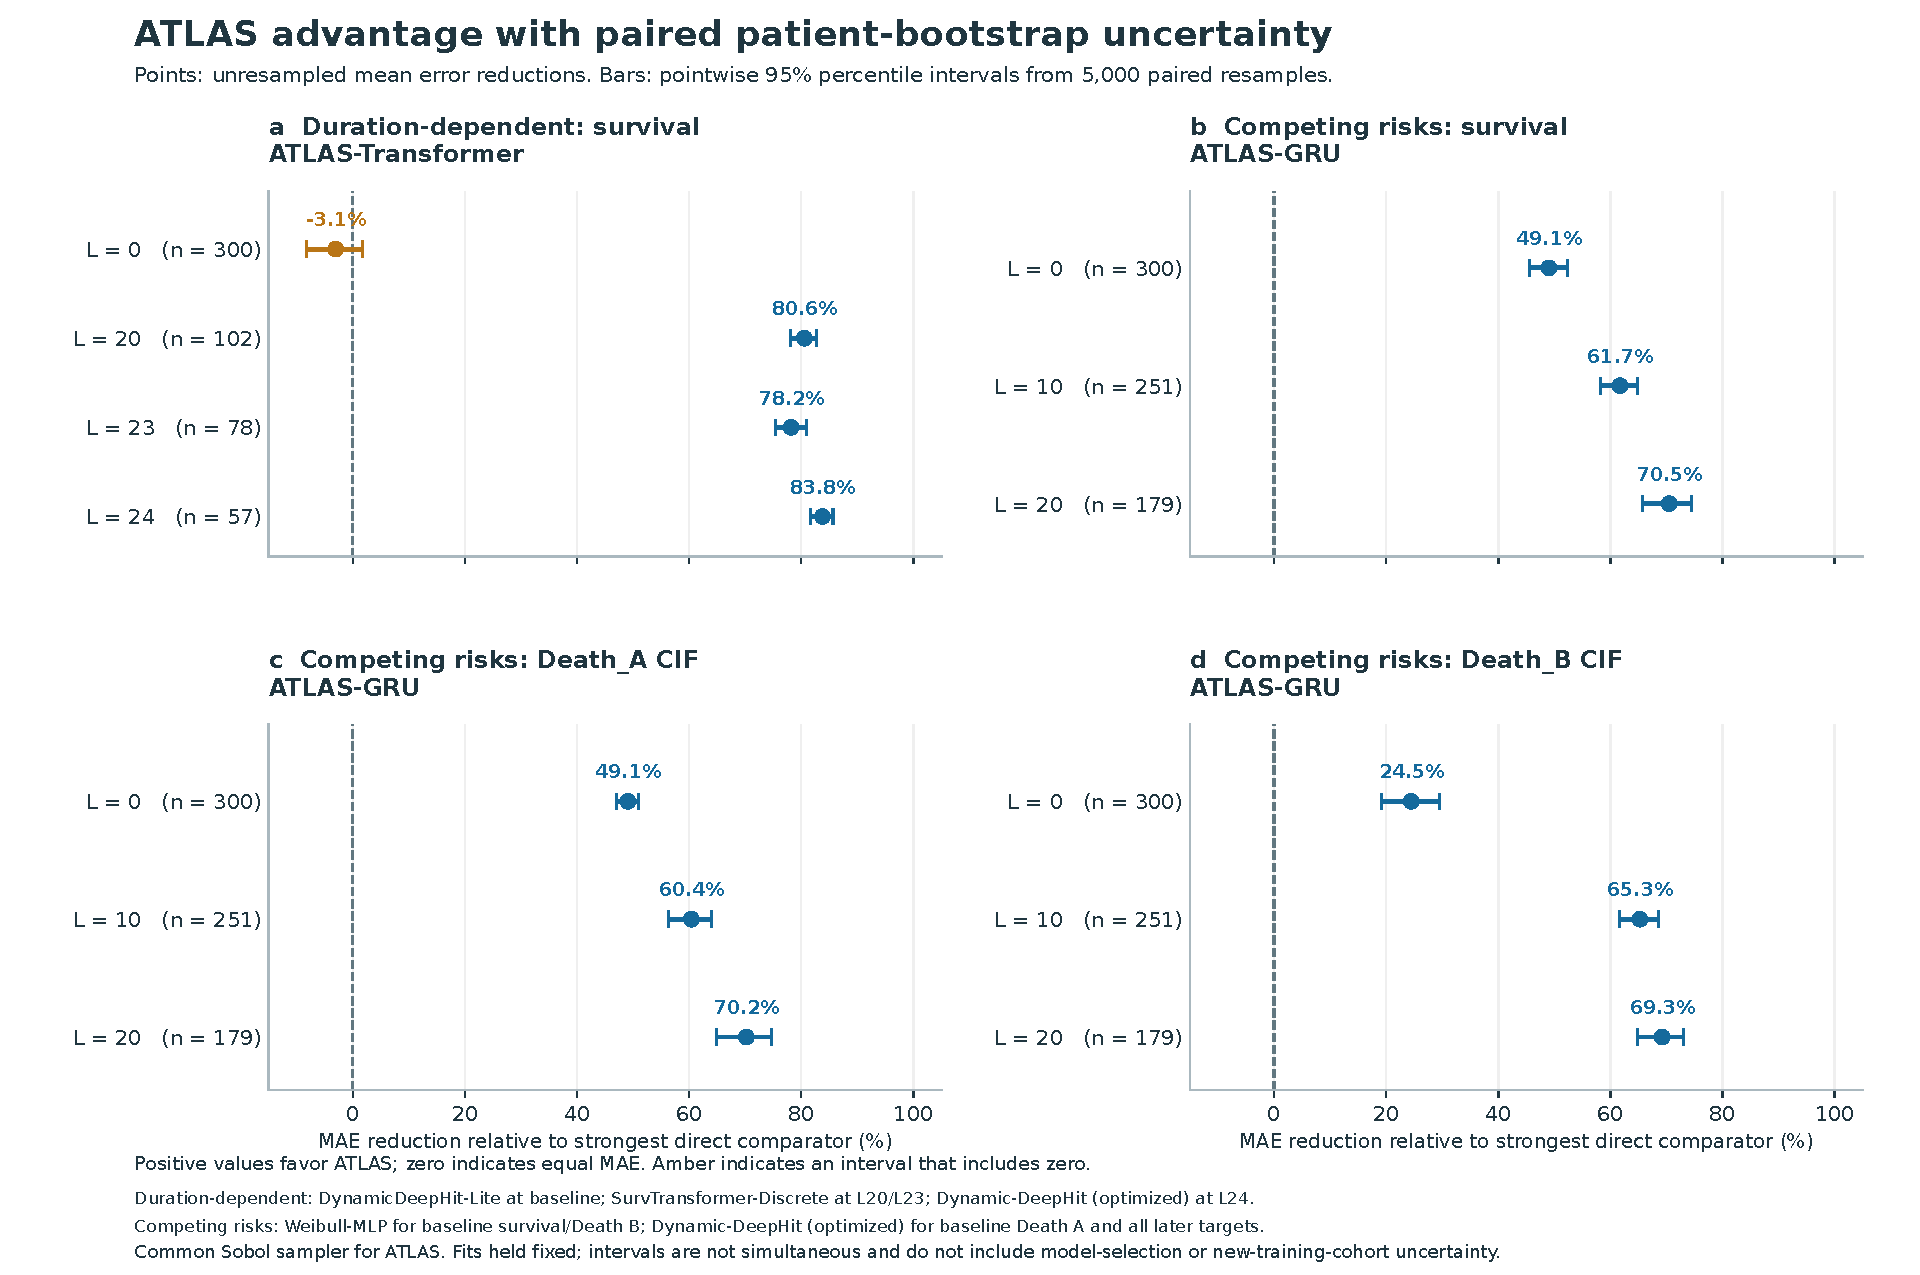
\includegraphics[width=\textwidth]{figures/figure_1_headline_bootstrap.pdf}
\caption{ATLAS-Transformer in the duration-dependent experiment and ATLAS-GRU in the competing-risks experiment are compared with the strongest fitted direct comparator at each landmark and target. Points show relative MAE reductions, 100 times (comparator MAE minus ATLAS MAE) divided by comparator MAE; positive values favor ATLAS. Bars are pointwise 95\% percentile intervals from 5,000 paired patient resamples. The duration-dependent comparators are DynamicDeepHit-Lite at baseline, SurvTransformer-Discrete at landmarks 20 and 23, and Dynamic-DeepHit (optimized) at landmark 24. In competing risks, Weibull-MLP is used for baseline survival and Death B incidence, and Dynamic-DeepHit (optimized) for baseline Death A incidence and all post-baseline targets. Amber marks an interval including zero. ATLAS uses the common Sobol sampler. Comparisons are fixed by the unresampled updated results; fits are held fixed and intervals do not account for model selection or multiplicity.}\label{fig:patientboot_1}
\end{figure}
\begin{figure}[p]\centering
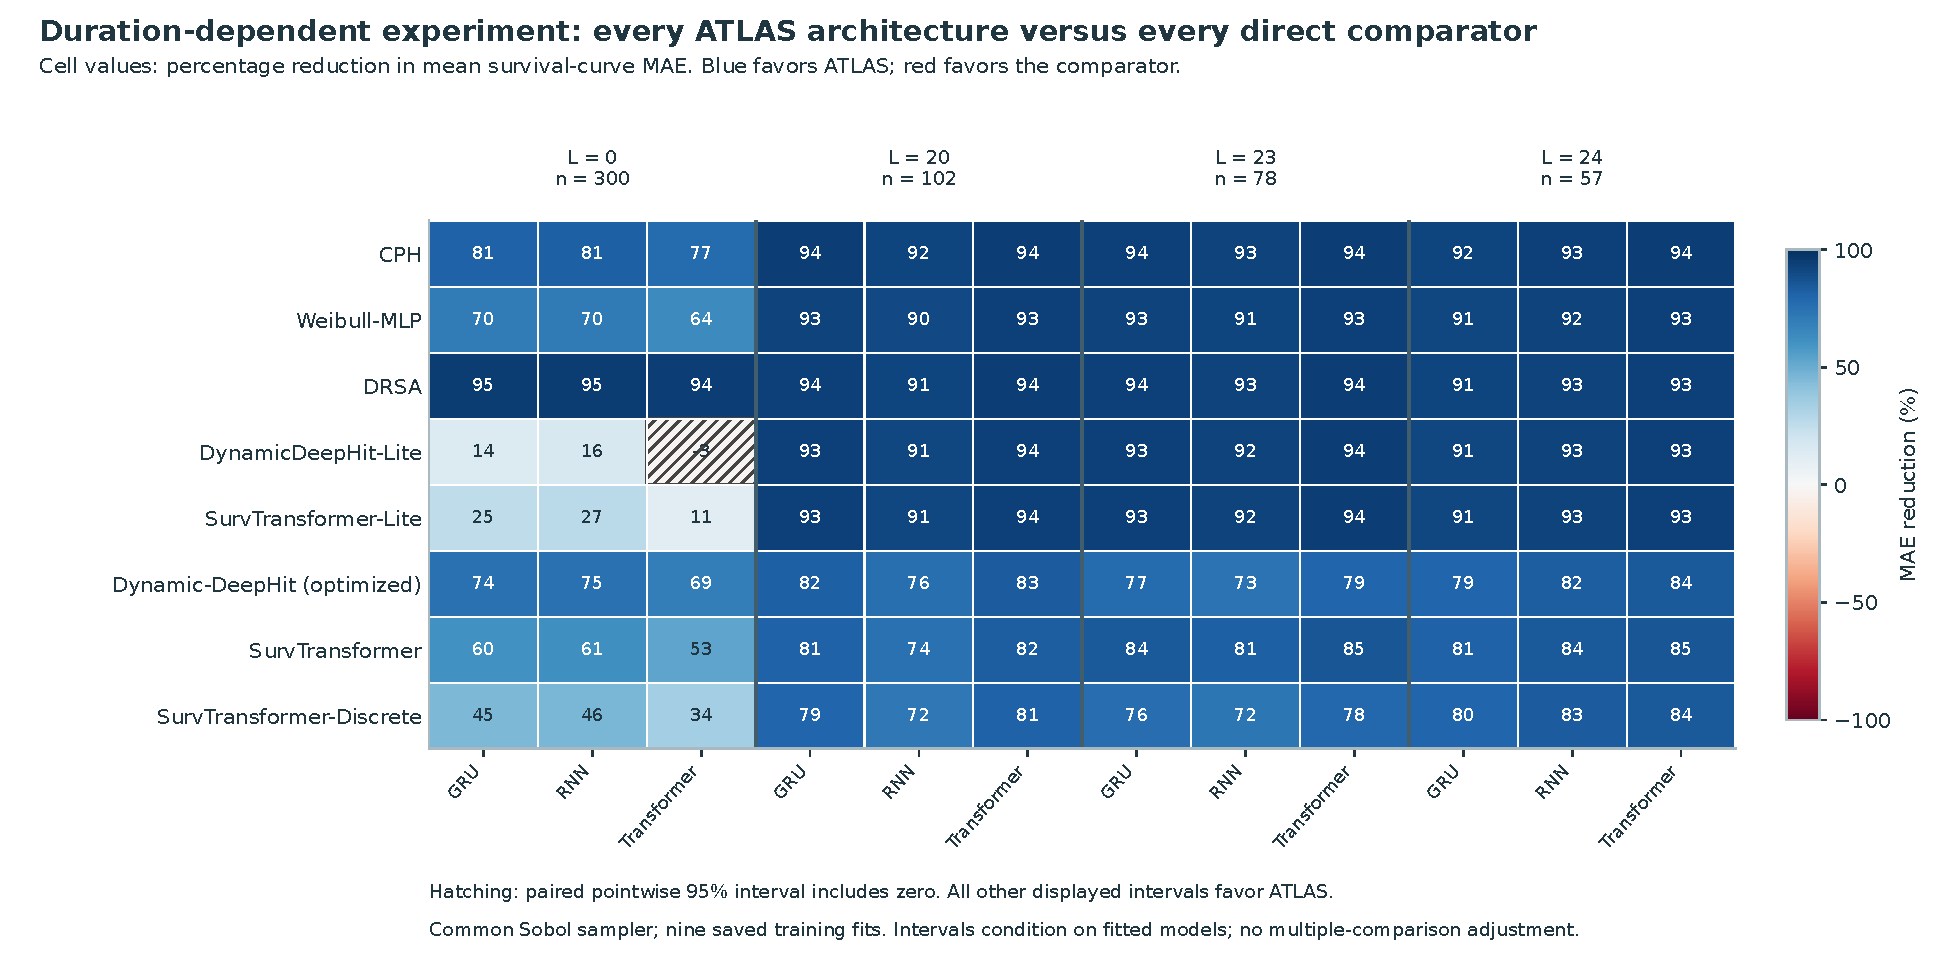
\includegraphics[width=\textwidth]{figures/figure_2_duration_comparator_matrix.pdf}
\caption{Cells show percentage reductions in mean survival-curve MAE for ATLAS-GRU, ATLAS-RNN and ATLAS-Transformer relative to each of the eight fitted direct comparators. Blue favors ATLAS and red favors the comparator; a common scale from -100\% to 100\% is centered at zero. Hatching marks a pointwise 95\% paired patient-bootstrap interval for the MAE difference that includes zero. This occurs only for baseline Transformer versus DynamicDeepHit-Lite. ATLAS means average common-Sobol errors over nine saved training fits. Cell values are rounded to whole percentages. Different eligible patient populations and prediction windows apply across landmarks; intervals are not simultaneous.}\label{fig:patientboot_2}
\end{figure}
\begin{figure}[p]\centering
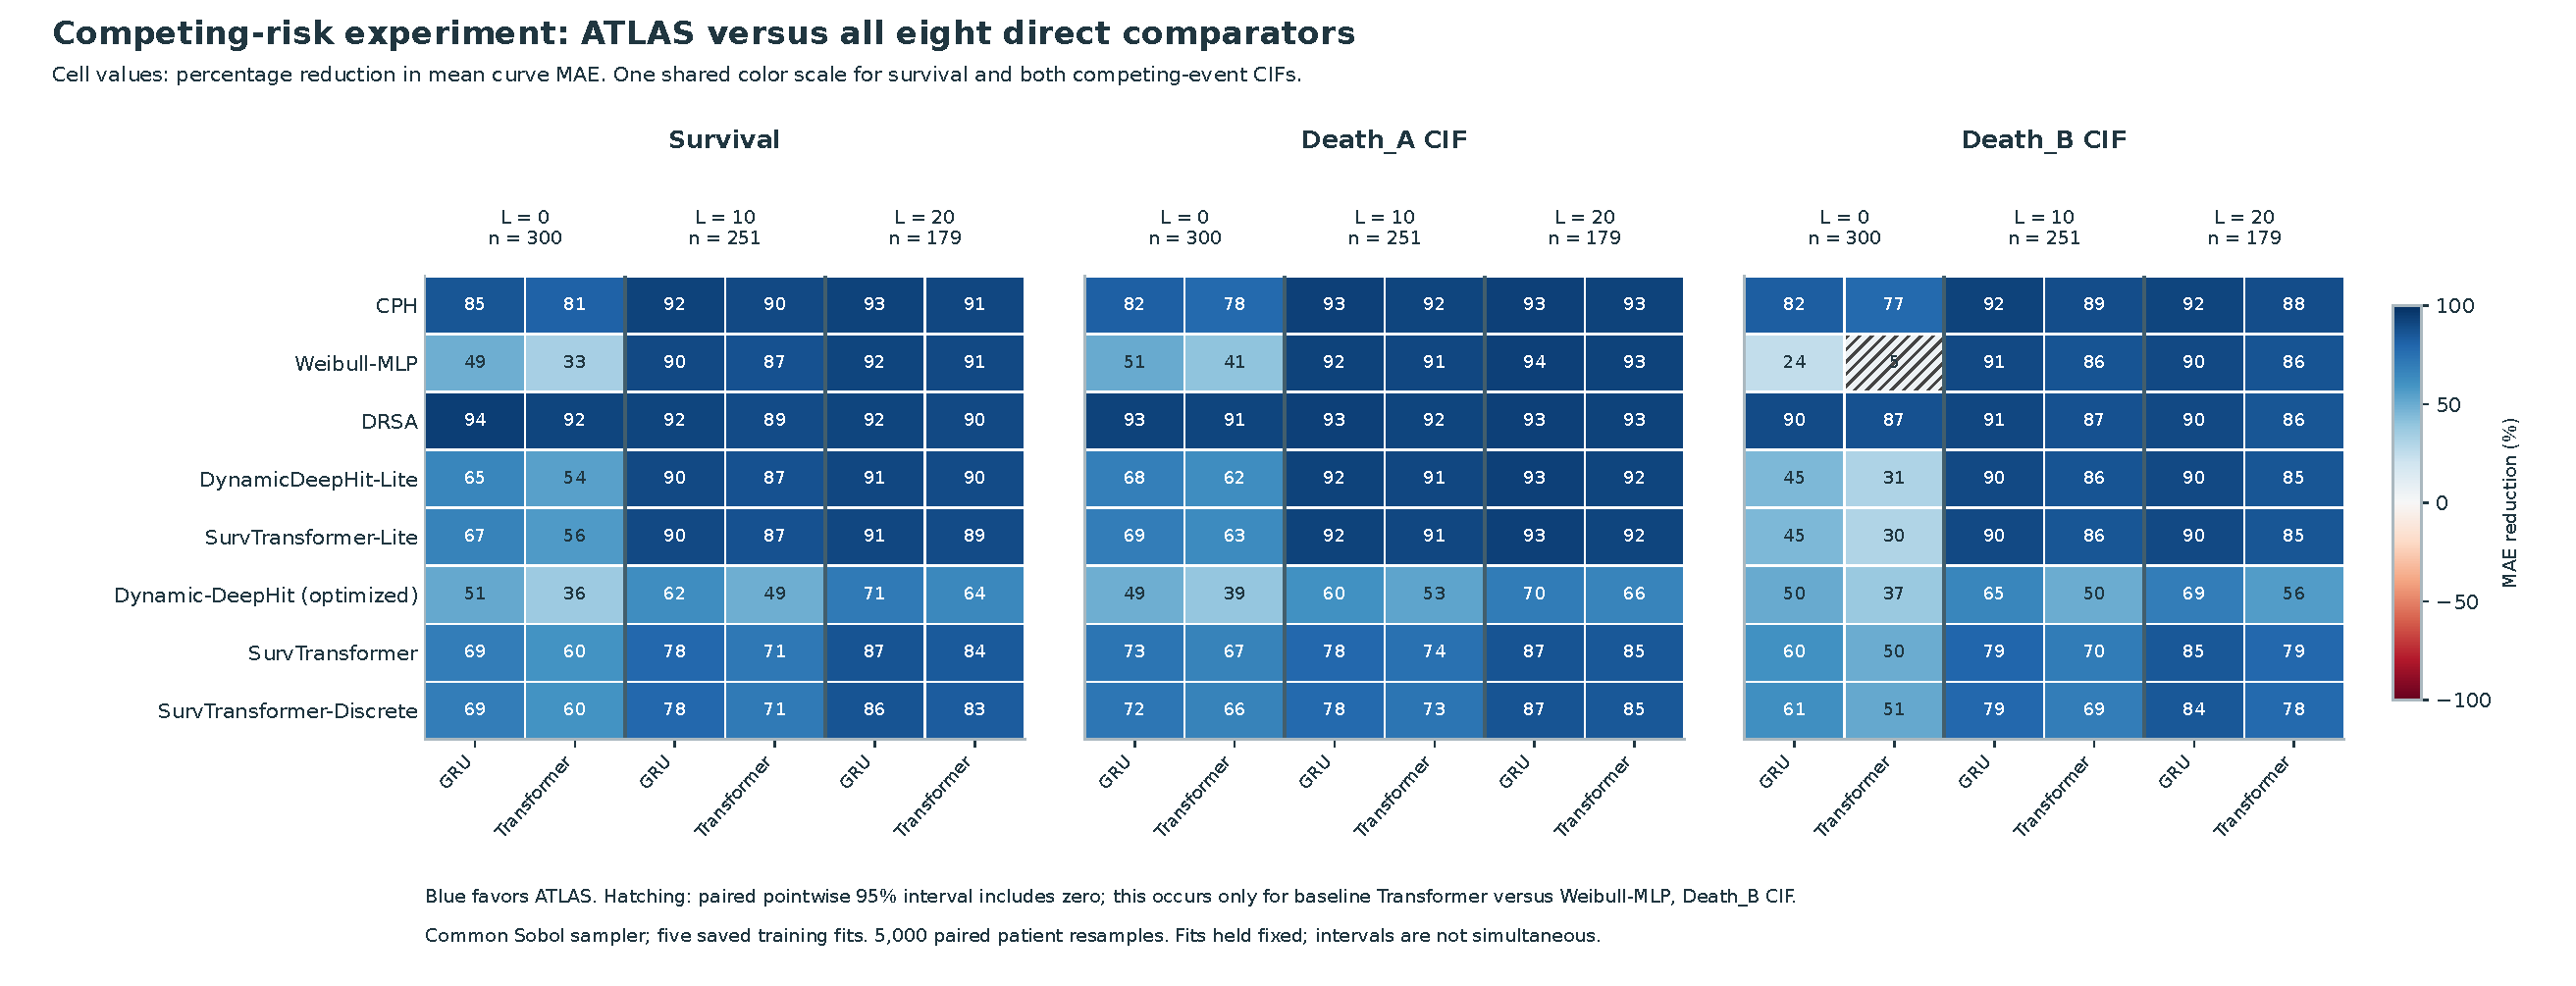
\includegraphics[width=\textwidth]{figures/figure_3_competing_risk_comparator_matrix.pdf}
\caption{The three panels show survival, Death A CIF and Death B CIF comparisons for ATLAS-GRU and ATLAS-Transformer against the eight fitted direct comparators. Cells show relative reductions in mean MAE with the same color scale and hatching convention as Figure~\ref{fig:patientboot_2}. All point estimates favor ATLAS, but the baseline Transformer versus Weibull-MLP Death B CIF interval includes zero. ATLAS means use the common Sobol sampler and five saved training fits. Errors and bootstrap resamples are paired by patient across models, landmarks and targets. These are pointwise intervals conditional on saved fits, without adjustment for multiple comparisons; percentage error reductions are not reductions in clinical event risk.}\label{fig:patientboot_3}
\end{figure}

\clearpage
\subsection{Complete numerical comparisons}
Table~\ref{tab:patientboot_all} reports all 240 comparisons. Architecture names identify ATLAS models using the common Sobol sampler. Targets S, A and B denote survival, Death A CIF and Death B CIF. Differences are ATLAS minus comparator MAE, with negative values favoring ATLAS; positive relative reductions favor ATLAS. Values in brackets are pointwise 95\% paired patient-bootstrap intervals. Comparator names identify the fitted models; Weibull denotes Weibull-MLP and Dynamic-DeepHit (optimized) denotes the validation-selected adaptation.
\begingroup\scriptsize
\setlength{\tabcolsep}{3pt}
\begin{longtable}{lll p{3.0cm} rr}
\caption{Complete paired patient-bootstrap comparisons. MAE differences retain the probability scale; relative reductions are percentages.}\label{tab:patientboot_all}\\
\toprule
ATLAS & L & Target & Comparator & Difference [95\% interval] & Reduction [95\% interval]\\\midrule
\endfirsthead
\multicolumn{6}{l}{\tablename~\thetable\ (continued)}\\\toprule
ATLAS & L & Target & Comparator & Difference [95\% interval] & Reduction [95\% interval]\\\midrule
\endhead
\bottomrule\endfoot
\multicolumn{6}{l}{\textbf{Duration-dependent experiment}}\\\midrule
GRU & 0 & S & CPH & -0.031475 [-0.034783, -0.028406] & 81.0 [79.4, 82.5]\\
GRU & 0 & S & Weibull-MLP & -0.016882 [-0.017068, -0.016704] & 69.6 [69.3, 69.9]\\
GRU & 0 & S & DRSA & -0.138893 [-0.140504, -0.137265] & 95.0 [94.9, 95.1]\\
GRU & 0 & S & DynamicDeepHit-Lite & -0.001186 [-0.001528, -0.000829] & 13.9 [10.0, 17.3]\\
GRU & 0 & S & SurvTransformer-Lite & -0.002506 [-0.002822, -0.002186] & 25.4 [22.8, 27.8]\\
GRU & 0 & S & Dynamic-DeepHit (optimized) & -0.021235 [-0.022451, -0.020027] & 74.2 [72.9, 75.4]\\
GRU & 0 & S & SurvTransformer & -0.011232 [-0.011862, -0.010644] & 60.4 [59.2, 61.6]\\
GRU & 0 & S & SurvTransformer-Discrete & -0.005925 [-0.006530, -0.005347] & 44.6 [42.1, 47.0]\\
RNN & 0 & S & CPH & -0.031650 [-0.034968, -0.028555] & 81.5 [79.9, 82.9]\\
RNN & 0 & S & Weibull-MLP & -0.017057 [-0.017303, -0.016812] & 70.3 [69.8, 70.9]\\
RNN & 0 & S & DRSA & -0.139067 [-0.140615, -0.137517] & 95.1 [95.0, 95.2]\\
RNN & 0 & S & DynamicDeepHit-Lite & -0.001360 [-0.001724, -0.000986] & 15.9 [11.9, 19.5]\\
RNN & 0 & S & SurvTransformer-Lite & -0.002681 [-0.002997, -0.002355] & 27.1 [24.5, 29.6]\\
RNN & 0 & S & Dynamic-DeepHit (optimized) & -0.021409 [-0.022555, -0.020263] & 74.8 [73.8, 75.8]\\
RNN & 0 & S & SurvTransformer & -0.011407 [-0.012066, -0.010790] & 61.3 [60.0, 62.7]\\
RNN & 0 & S & SurvTransformer-Discrete & -0.006100 [-0.006721, -0.005504] & 45.9 [43.3, 48.3]\\
Transformer & 0 & S & CPH & -0.030027 [-0.033193, -0.027056] & 77.3 [75.7, 78.7]\\
Transformer & 0 & S & Weibull-MLP & -0.015435 [-0.015663, -0.015212] & 63.6 [62.8, 64.4]\\
Transformer & 0 & S & DRSA & -0.137445 [-0.139098, -0.135804] & 94.0 [93.8, 94.1]\\
Transformer & 0 & S & DynamicDeepHit-Lite & 0.000262 [-0.000146, 0.000685] & -3.1 [-8.3, 1.6]\\
Transformer & 0 & S & SurvTransformer-Lite & -0.001059 [-0.001395, -0.000715] & 10.7 [7.4, 13.8]\\
Transformer & 0 & S & Dynamic-DeepHit (optimized) & -0.019787 [-0.021036, -0.018567] & 69.2 [67.5, 70.7]\\
Transformer & 0 & S & SurvTransformer & -0.009785 [-0.010344, -0.009256] & 52.6 [51.3, 53.9]\\
Transformer & 0 & S & SurvTransformer-Discrete & -0.004478 [-0.005025, -0.003955] & 33.7 [30.9, 36.3]\\
GRU & 20 & S & CPH & -0.148154 [-0.168786, -0.129227] & 93.8 [92.8, 94.7]\\
GRU & 20 & S & Weibull-MLP & -0.127261 [-0.148976, -0.107806] & 92.9 [91.5, 94.1]\\
GRU & 20 & S & DRSA & -0.142925 [-0.158622, -0.128706] & 93.6 [92.7, 94.4]\\
GRU & 20 & S & DynamicDeepHit-Lite & -0.132828 [-0.150728, -0.117009] & 93.2 [92.1, 94.2]\\
GRU & 20 & S & SurvTransformer-Lite & -0.132497 [-0.150878, -0.116336] & 93.1 [92.0, 94.2]\\
GRU & 20 & S & Dynamic-DeepHit (optimized) & -0.043980 [-0.051081, -0.037115] & 81.8 [79.0, 84.1]\\
GRU & 20 & S & SurvTransformer & -0.041137 [-0.046600, -0.036182] & 80.8 [78.2, 83.2]\\
GRU & 20 & S & SurvTransformer-Discrete & -0.036778 [-0.041082, -0.032795] & 79.0 [76.6, 81.1]\\
RNN & 20 & S & CPH & -0.144804 [-0.165515, -0.125996] & 91.7 [90.3, 92.9]\\
RNN & 20 & S & Weibull-MLP & -0.123911 [-0.145487, -0.104406] & 90.4 [88.6, 92.0]\\
RNN & 20 & S & DRSA & -0.139575 [-0.155277, -0.125499] & 91.4 [90.3, 92.5]\\
RNN & 20 & S & DynamicDeepHit-Lite & -0.129478 [-0.147370, -0.113640] & 90.8 [89.5, 92.1]\\
RNN & 20 & S & SurvTransformer-Lite & -0.129147 [-0.147521, -0.113013] & 90.8 [89.4, 92.1]\\
RNN & 20 & S & Dynamic-DeepHit (optimized) & -0.040630 [-0.047686, -0.033848] & 75.6 [71.8, 78.5]\\
RNN & 20 & S & SurvTransformer & -0.037786 [-0.043316, -0.032730] & 74.2 [70.9, 77.3]\\
RNN & 20 & S & SurvTransformer-Discrete & -0.033428 [-0.037597, -0.029587] & 71.8 [69.0, 74.3]\\
Transformer & 20 & S & CPH & -0.148876 [-0.169278, -0.130193] & 94.3 [93.4, 95.1]\\
Transformer & 20 & S & Weibull-MLP & -0.127984 [-0.149552, -0.108670] & 93.4 [92.1, 94.5]\\
Transformer & 20 & S & DRSA & -0.143648 [-0.159322, -0.129507] & 94.1 [93.2, 94.9]\\
Transformer & 20 & S & DynamicDeepHit-Lite & -0.133550 [-0.151199, -0.117659] & 93.7 [92.6, 94.6]\\
Transformer & 20 & S & SurvTransformer-Lite & -0.133220 [-0.151385, -0.117229] & 93.6 [92.6, 94.6]\\
Transformer & 20 & S & Dynamic-DeepHit (optimized) & -0.044702 [-0.051662, -0.037999] & 83.2 [80.7, 85.2]\\
Transformer & 20 & S & SurvTransformer & -0.041859 [-0.047185, -0.036969] & 82.2 [79.7, 84.5]\\
Transformer & 20 & S & SurvTransformer-Discrete & -0.037501 [-0.041791, -0.033499] & 80.6 [78.1, 82.8]\\
GRU & 23 & S & CPH & -0.198253 [-0.220212, -0.177872] & 93.6 [92.7, 94.4]\\
GRU & 23 & S & Weibull-MLP & -0.172119 [-0.206457, -0.138461] & 92.7 [91.1, 93.9]\\
GRU & 23 & S & DRSA & -0.200157 [-0.217583, -0.184167] & 93.6 [92.8, 94.4]\\
GRU & 23 & S & DynamicDeepHit-Lite & -0.191104 [-0.210697, -0.173406] & 93.3 [92.5, 94.1]\\
GRU & 23 & S & SurvTransformer-Lite & -0.190595 [-0.210256, -0.172648] & 93.3 [92.5, 94.1]\\
GRU & 23 & S & Dynamic-DeepHit (optimized) & -0.046195 [-0.052315, -0.040429] & 77.2 [75.1, 79.1]\\
GRU & 23 & S & SurvTransformer & -0.071642 [-0.083159, -0.061043] & 84.0 [81.6, 86.2]\\
GRU & 23 & S & SurvTransformer-Discrete & -0.043848 [-0.048405, -0.039422] & 76.3 [73.3, 78.9]\\
RNN & 23 & S & CPH & -0.196011 [-0.217650, -0.175723] & 92.5 [91.4, 93.5]\\
RNN & 23 & S & Weibull-MLP & -0.169877 [-0.203812, -0.136718] & 91.4 [89.8, 92.7]\\
RNN & 23 & S & DRSA & -0.197915 [-0.215497, -0.181709] & 92.6 [91.5, 93.6]\\
RNN & 23 & S & DynamicDeepHit-Lite & -0.188862 [-0.208488, -0.170938] & 92.2 [91.1, 93.3]\\
RNN & 23 & S & SurvTransformer-Lite & -0.188354 [-0.207942, -0.170365] & 92.2 [91.1, 93.3]\\
RNN & 23 & S & Dynamic-DeepHit (optimized) & -0.043953 [-0.049672, -0.038543] & 73.4 [70.8, 75.8]\\
RNN & 23 & S & SurvTransformer & -0.069400 [-0.080960, -0.058928] & 81.4 [78.4, 84.1]\\
RNN & 23 & S & SurvTransformer-Discrete & -0.041606 [-0.046294, -0.037043] & 72.4 [68.4, 75.9]\\
Transformer & 23 & S & CPH & -0.199375 [-0.221213, -0.179032] & 94.1 [93.2, 94.9]\\
Transformer & 23 & S & Weibull-MLP & -0.173241 [-0.207110, -0.140071] & 93.3 [92.0, 94.2]\\
Transformer & 23 & S & DRSA & -0.201279 [-0.218611, -0.185308] & 94.1 [93.3, 94.9]\\
Transformer & 23 & S & DynamicDeepHit-Lite & -0.192226 [-0.211599, -0.174476] & 93.9 [93.0, 94.6]\\
Transformer & 23 & S & SurvTransformer-Lite & -0.191717 [-0.211078, -0.173967] & 93.9 [93.0, 94.6]\\
Transformer & 23 & S & Dynamic-DeepHit (optimized) & -0.047317 [-0.053246, -0.041569] & 79.1 [76.9, 81.0]\\
Transformer & 23 & S & SurvTransformer & -0.072763 [-0.083890, -0.062557] & 85.3 [83.3, 87.2]\\
Transformer & 23 & S & SurvTransformer-Discrete & -0.044970 [-0.049395, -0.040651] & 78.2 [75.4, 81.0]\\
GRU & 24 & S & CPH & -0.158125 [-0.186520, -0.132199] & 92.1 [90.6, 93.3]\\
GRU & 24 & S & Weibull-MLP & -0.137082 [-0.168547, -0.108566] & 91.0 [89.0, 92.5]\\
GRU & 24 & S & DRSA & -0.146135 [-0.171423, -0.122199] & 91.5 [89.9, 92.7]\\
GRU & 24 & S & DynamicDeepHit-Lite & -0.141634 [-0.168859, -0.116279] & 91.2 [89.5, 92.6]\\
GRU & 24 & S & SurvTransformer-Lite & -0.142583 [-0.170008, -0.117227] & 91.3 [89.6, 92.6]\\
GRU & 24 & S & Dynamic-DeepHit (optimized) & -0.051175 [-0.061379, -0.041556] & 79.0 [76.2, 81.4]\\
GRU & 24 & S & SurvTransformer & -0.057890 [-0.066434, -0.050214] & 81.0 [78.7, 83.1]\\
GRU & 24 & S & SurvTransformer-Discrete & -0.053342 [-0.059781, -0.047407] & 79.7 [77.1, 82.2]\\
RNN & 24 & S & CPH & -0.160249 [-0.189083, -0.133990] & 93.3 [91.8, 94.5]\\
RNN & 24 & S & Weibull-MLP & -0.139207 [-0.170737, -0.110504] & 92.4 [90.5, 93.8]\\
RNN & 24 & S & DRSA & -0.148260 [-0.173856, -0.124180] & 92.8 [91.4, 94.0]\\
RNN & 24 & S & DynamicDeepHit-Lite & -0.143759 [-0.171329, -0.118078] & 92.6 [91.0, 93.9]\\
RNN & 24 & S & SurvTransformer-Lite & -0.144708 [-0.171965, -0.119044] & 92.6 [91.1, 93.9]\\
RNN & 24 & S & Dynamic-DeepHit (optimized) & -0.053300 [-0.064125, -0.043043] & 82.3 [78.9, 85.0]\\
RNN & 24 & S & SurvTransformer & -0.060015 [-0.068871, -0.051920] & 83.9 [81.3, 86.1]\\
RNN & 24 & S & SurvTransformer-Discrete & -0.055467 [-0.061896, -0.049464] & 82.8 [80.3, 85.0]\\
Transformer & 24 & S & CPH & -0.161247 [-0.190084, -0.134776] & 93.9 [92.4, 95.0]\\
Transformer & 24 & S & Weibull-MLP & -0.140204 [-0.171871, -0.111647] & 93.0 [91.1, 94.4]\\
Transformer & 24 & S & DRSA & -0.149258 [-0.174889, -0.124817] & 93.4 [91.7, 94.6]\\
Transformer & 24 & S & DynamicDeepHit-Lite & -0.144757 [-0.172341, -0.119006] & 93.2 [91.5, 94.5]\\
Transformer & 24 & S & SurvTransformer-Lite & -0.145706 [-0.172996, -0.119954] & 93.3 [91.5, 94.5]\\
Transformer & 24 & S & Dynamic-DeepHit (optimized) & -0.054298 [-0.064475, -0.044688] & 83.8 [81.7, 85.7]\\
Transformer & 24 & S & SurvTransformer & -0.061013 [-0.069266, -0.053500] & 85.3 [83.2, 87.1]\\
Transformer & 24 & S & SurvTransformer-Discrete & -0.056465 [-0.062487, -0.050947] & 84.3 [82.1, 86.4]\\
\multicolumn{6}{l}{\textbf{Competing-risks experiment}}\\\midrule
GRU & 0 & S & CPH & -0.046281 [-0.049271, -0.043216] & 85.4 [84.4, 86.4]\\
GRU & 0 & S & Weibull-MLP & -0.007608 [-0.008439, -0.006784] & 49.1 [45.6, 52.3]\\
GRU & 0 & S & DRSA & -0.123379 [-0.128451, -0.118167] & 94.0 [93.6, 94.4]\\
GRU & 0 & S & DynamicDeepHit-Lite & -0.014804 [-0.016700, -0.012929] & 65.2 [61.9, 68.1]\\
GRU & 0 & S & SurvTransformer-Lite & -0.015952 [-0.017955, -0.014049] & 66.9 [63.7, 69.6]\\
GRU & 0 & S & Dynamic-DeepHit (optimized) & -0.008340 [-0.009127, -0.007591] & 51.3 [48.8, 53.8]\\
GRU & 0 & S & SurvTransformer & -0.017784 [-0.018860, -0.016750] & 69.2 [67.3, 71.1]\\
GRU & 0 & S & SurvTransformer-Discrete & -0.017876 [-0.018875, -0.016890] & 69.3 [67.7, 71.0]\\
Transformer & 0 & S & CPH & -0.043805 [-0.047038, -0.040474] & 80.8 [79.2, 82.4]\\
Transformer & 0 & S & Weibull-MLP & -0.005132 [-0.006075, -0.004179] & 33.1 [28.0, 37.5]\\
Transformer & 0 & S & DRSA & -0.120902 [-0.125783, -0.115882] & 92.1 [91.7, 92.5]\\
Transformer & 0 & S & DynamicDeepHit-Lite & -0.012327 [-0.014194, -0.010420] & 54.3 [50.1, 57.9]\\
Transformer & 0 & S & SurvTransformer-Lite & -0.013475 [-0.015459, -0.011500] & 56.5 [52.4, 59.9]\\
Transformer & 0 & S & Dynamic-DeepHit (optimized) & -0.005864 [-0.006742, -0.005042] & 36.1 [32.5, 39.6]\\
Transformer & 0 & S & SurvTransformer & -0.015308 [-0.016384, -0.014332] & 59.6 [57.5, 61.7]\\
Transformer & 0 & S & SurvTransformer-Discrete & -0.015399 [-0.016492, -0.014357] & 59.7 [57.6, 62.0]\\
GRU & 0 & A & CPH & -0.026439 [-0.028898, -0.024139] & 81.8 [80.4, 83.0]\\
GRU & 0 & A & Weibull-MLP & -0.006063 [-0.006799, -0.005340] & 50.8 [47.4, 53.8]\\
GRU & 0 & A & DRSA & -0.077184 [-0.081081, -0.073311] & 92.9 [92.4, 93.4]\\
GRU & 0 & A & DynamicDeepHit-Lite & -0.012760 [-0.014701, -0.010832] & 68.5 [65.1, 71.2]\\
GRU & 0 & A & SurvTransformer-Lite & -0.013299 [-0.015202, -0.011407] & 69.3 [66.1, 72.1]\\
GRU & 0 & A & Dynamic-DeepHit (optimized) & -0.005667 [-0.006209, -0.005160] & 49.1 [47.1, 50.9]\\
GRU & 0 & A & SurvTransformer & -0.015697 [-0.016602, -0.014829] & 72.8 [71.1, 74.4]\\
GRU & 0 & A & SurvTransformer-Discrete & -0.015273 [-0.016281, -0.014272] & 72.2 [70.8, 73.6]\\
Transformer & 0 & A & CPH & -0.025227 [-0.027972, -0.022708] & 78.1 [75.8, 80.1]\\
Transformer & 0 & A & Weibull-MLP & -0.004850 [-0.005728, -0.004023] & 40.6 [36.1, 44.9]\\
Transformer & 0 & A & DRSA & -0.075972 [-0.079812, -0.072192] & 91.5 [91.1, 91.8]\\
Transformer & 0 & A & DynamicDeepHit-Lite & -0.011547 [-0.013592, -0.009535] & 62.0 [57.5, 65.7]\\
Transformer & 0 & A & SurvTransformer-Lite & -0.012087 [-0.014103, -0.010111] & 63.0 [58.9, 66.6]\\
Transformer & 0 & A & Dynamic-DeepHit (optimized) & -0.004455 [-0.005229, -0.003748] & 38.6 [34.5, 42.5]\\
Transformer & 0 & A & SurvTransformer & -0.014485 [-0.015432, -0.013579] & 67.1 [65.5, 68.7]\\
Transformer & 0 & A & SurvTransformer-Discrete & -0.014061 [-0.015224, -0.012960] & 66.5 [64.5, 68.4]\\
GRU & 0 & B & CPH & -0.022580 [-0.024310, -0.020824] & 82.0 [80.7, 83.3]\\
GRU & 0 & B & Weibull-MLP & -0.001602 [-0.002041, -0.001190] & 24.5 [19.2, 29.5]\\
GRU & 0 & B & DRSA & -0.043284 [-0.046300, -0.040288] & 89.8 [89.1, 90.3]\\
GRU & 0 & B & DynamicDeepHit-Lite & -0.004053 [-0.005049, -0.003121] & 45.1 [38.9, 50.1]\\
GRU & 0 & B & SurvTransformer-Lite & -0.003989 [-0.004757, -0.003232] & 44.7 [39.8, 48.8]\\
GRU & 0 & B & Dynamic-DeepHit (optimized) & -0.004971 [-0.005427, -0.004532] & 50.2 [47.8, 52.5]\\
GRU & 0 & B & SurvTransformer & -0.007481 [-0.008187, -0.006792] & 60.2 [57.9, 62.4]\\
GRU & 0 & B & SurvTransformer-Discrete & -0.007713 [-0.008330, -0.007102] & 61.0 [58.9, 62.9]\\
Transformer & 0 & B & CPH & -0.021309 [-0.022960, -0.019583] & 77.4 [75.9, 78.9]\\
Transformer & 0 & B & Weibull-MLP & -0.000331 [-0.000773, 0.000104] & 5.1 [-1.6, 11.2]\\
Transformer & 0 & B & DRSA & -0.042014 [-0.044971, -0.039105] & 87.1 [86.5, 87.7]\\
Transformer & 0 & B & DynamicDeepHit-Lite & -0.002782 [-0.003742, -0.001894] & 30.9 [23.7, 37.2]\\
Transformer & 0 & B & SurvTransformer-Lite & -0.002718 [-0.003462, -0.001987] & 30.4 [24.3, 35.6]\\
Transformer & 0 & B & Dynamic-DeepHit (optimized) & -0.003701 [-0.004145, -0.003275] & 37.3 [34.4, 40.2]\\
Transformer & 0 & B & SurvTransformer & -0.006210 [-0.006832, -0.005609] & 50.0 [47.7, 52.2]\\
Transformer & 0 & B & SurvTransformer-Discrete & -0.006442 [-0.007011, -0.005901] & 50.9 [48.8, 53.0]\\
GRU & 10 & S & CPH & -0.106974 [-0.117243, -0.097523] & 92.4 [91.5, 93.2]\\
GRU & 10 & S & Weibull-MLP & -0.081152 [-0.091051, -0.071408] & 90.2 [89.0, 91.2]\\
GRU & 10 & S & DRSA & -0.099898 [-0.109319, -0.090508] & 91.9 [90.8, 92.8]\\
GRU & 10 & S & DynamicDeepHit-Lite & -0.082591 [-0.092225, -0.072883] & 90.3 [89.1, 91.4]\\
GRU & 10 & S & SurvTransformer-Lite & -0.081760 [-0.091450, -0.071897] & 90.3 [89.0, 91.3]\\
GRU & 10 & S & Dynamic-DeepHit (optimized) & -0.014236 [-0.015992, -0.012561] & 61.7 [58.3, 64.8]\\
GRU & 10 & S & SurvTransformer & -0.031780 [-0.035839, -0.028036] & 78.3 [75.9, 80.5]\\
GRU & 10 & S & SurvTransformer-Discrete & -0.031639 [-0.035310, -0.028146] & 78.2 [75.9, 80.2]\\
Transformer & 10 & S & CPH & -0.104072 [-0.114470, -0.094505] & 89.9 [88.7, 90.9]\\
Transformer & 10 & S & Weibull-MLP & -0.078249 [-0.088064, -0.068535] & 87.0 [85.4, 88.3]\\
Transformer & 10 & S & DRSA & -0.096996 [-0.106426, -0.087654] & 89.2 [87.9, 90.4]\\
Transformer & 10 & S & DynamicDeepHit-Lite & -0.079688 [-0.089372, -0.069991] & 87.2 [85.6, 88.5]\\
Transformer & 10 & S & SurvTransformer-Lite & -0.078857 [-0.088568, -0.069135] & 87.1 [85.5, 88.4]\\
Transformer & 10 & S & Dynamic-DeepHit (optimized) & -0.011334 [-0.013054, -0.009696] & 49.1 [45.0, 52.9]\\
Transformer & 10 & S & SurvTransformer & -0.028877 [-0.032871, -0.025198] & 71.1 [68.2, 73.8]\\
Transformer & 10 & S & SurvTransformer-Discrete & -0.028737 [-0.032337, -0.025329] & 71.0 [68.4, 73.5]\\
GRU & 10 & A & CPH & -0.094703 [-0.104863, -0.085399] & 93.1 [92.3, 93.8]\\
GRU & 10 & A & Weibull-MLP & -0.084648 [-0.094257, -0.075459] & 92.3 [91.5, 93.0]\\
GRU & 10 & A & DRSA & -0.095192 [-0.104559, -0.086164] & 93.1 [92.2, 93.9]\\
GRU & 10 & A & DynamicDeepHit-Lite & -0.085922 [-0.095742, -0.076496] & 92.4 [91.6, 93.1]\\
GRU & 10 & A & SurvTransformer-Lite & -0.085240 [-0.095116, -0.075747] & 92.4 [91.5, 93.1]\\
GRU & 10 & A & Dynamic-DeepHit (optimized) & -0.010763 [-0.012401, -0.009266] & 60.4 [56.4, 64.0]\\
GRU & 10 & A & SurvTransformer & -0.025738 [-0.029212, -0.022507] & 78.5 [76.1, 80.7]\\
GRU & 10 & A & SurvTransformer-Discrete & -0.024586 [-0.028062, -0.021305] & 77.7 [75.1, 80.0]\\
Transformer & 10 & A & CPH & -0.093336 [-0.103486, -0.084002] & 91.7 [90.9, 92.5]\\
Transformer & 10 & A & Weibull-MLP & -0.083281 [-0.092922, -0.074053] & 90.8 [89.9, 91.6]\\
Transformer & 10 & A & DRSA & -0.093825 [-0.103178, -0.084831] & 91.8 [90.8, 92.6]\\
Transformer & 10 & A & DynamicDeepHit-Lite & -0.084555 [-0.094356, -0.075075] & 90.9 [90.0, 91.8]\\
Transformer & 10 & A & SurvTransformer-Lite & -0.083873 [-0.093721, -0.074379] & 90.9 [90.0, 91.7]\\
Transformer & 10 & A & Dynamic-DeepHit (optimized) & -0.009396 [-0.011015, -0.007935] & 52.7 [48.7, 56.5]\\
Transformer & 10 & A & SurvTransformer & -0.024371 [-0.027789, -0.021151] & 74.3 [71.8, 76.7]\\
Transformer & 10 & A & SurvTransformer-Discrete & -0.023219 [-0.026698, -0.019969] & 73.4 [70.7, 76.0]\\
GRU & 10 & B & CPH & -0.051976 [-0.058860, -0.045857] & 92.4 [91.4, 93.2]\\
GRU & 10 & B & Weibull-MLP & -0.041295 [-0.047441, -0.035586] & 90.6 [89.3, 91.7]\\
GRU & 10 & B & DRSA & -0.045043 [-0.051206, -0.039033] & 91.3 [89.9, 92.5]\\
GRU & 10 & B & DynamicDeepHit-Lite & -0.039958 [-0.046107, -0.034170] & 90.3 [89.0, 91.5]\\
GRU & 10 & B & SurvTransformer-Lite & -0.039722 [-0.045823, -0.033936] & 90.2 [88.9, 91.4]\\
GRU & 10 & B & Dynamic-DeepHit (optimized) & -0.008086 [-0.009554, -0.006745] & 65.3 [61.6, 68.5]\\
GRU & 10 & B & SurvTransformer & -0.016495 [-0.019411, -0.013872] & 79.3 [76.6, 81.7]\\
GRU & 10 & B & SurvTransformer-Discrete & -0.016068 [-0.018809, -0.013564] & 78.9 [76.1, 81.3]\\
Transformer & 10 & B & CPH & -0.050057 [-0.056652, -0.044072] & 89.0 [87.7, 90.1]\\
Transformer & 10 & B & Weibull-MLP & -0.039376 [-0.045385, -0.033831] & 86.4 [84.7, 87.9]\\
Transformer & 10 & B & DRSA & -0.043124 [-0.049191, -0.037251] & 87.4 [85.5, 89.1]\\
Transformer & 10 & B & DynamicDeepHit-Lite & -0.038039 [-0.044071, -0.032450] & 86.0 [84.1, 87.6]\\
Transformer & 10 & B & SurvTransformer-Lite & -0.037803 [-0.043791, -0.032138] & 85.9 [84.1, 87.5]\\
Transformer & 10 & B & Dynamic-DeepHit (optimized) & -0.006167 [-0.007486, -0.004990] & 49.8 [45.2, 54.0]\\
Transformer & 10 & B & SurvTransformer & -0.014576 [-0.017294, -0.012092] & 70.1 [66.7, 73.1]\\
Transformer & 10 & B & SurvTransformer-Discrete & -0.014149 [-0.016772, -0.011823] & 69.5 [66.0, 72.4]\\
GRU & 20 & S & CPH & -0.086375 [-0.098142, -0.075017] & 92.8 [91.5, 93.9]\\
GRU & 20 & S & Weibull-MLP & -0.078665 [-0.090022, -0.068056] & 92.1 [90.6, 93.4]\\
GRU & 20 & S & DRSA & -0.075708 [-0.086524, -0.065227] & 91.9 [90.4, 93.1]\\
GRU & 20 & S & DynamicDeepHit-Lite & -0.070665 [-0.082192, -0.059401] & 91.3 [89.8, 92.6]\\
GRU & 20 & S & SurvTransformer-Lite & -0.069957 [-0.081749, -0.058434] & 91.3 [89.7, 92.5]\\
GRU & 20 & S & Dynamic-DeepHit (optimized) & -0.016049 [-0.018552, -0.013629] & 70.5 [65.7, 74.5]\\
GRU & 20 & S & SurvTransformer & -0.043766 [-0.051553, -0.036586] & 86.7 [84.2, 88.8]\\
GRU & 20 & S & SurvTransformer-Discrete & -0.042237 [-0.050136, -0.035123] & 86.3 [83.5, 88.6]\\
Transformer & 20 & S & CPH & -0.084985 [-0.096794, -0.073741] & 91.3 [89.9, 92.5]\\
Transformer & 20 & S & Weibull-MLP & -0.077274 [-0.088470, -0.066578] & 90.5 [88.8, 92.0]\\
Transformer & 20 & S & DRSA & -0.074318 [-0.084979, -0.063801] & 90.2 [88.5, 91.6]\\
Transformer & 20 & S & DynamicDeepHit-Lite & -0.069275 [-0.080863, -0.057945] & 89.5 [87.7, 91.0]\\
Transformer & 20 & S & SurvTransformer-Lite & -0.068567 [-0.080301, -0.057098] & 89.4 [87.6, 91.0]\\
Transformer & 20 & S & Dynamic-DeepHit (optimized) & -0.014658 [-0.017134, -0.012296] & 64.4 [59.2, 68.9]\\
Transformer & 20 & S & SurvTransformer & -0.042375 [-0.050017, -0.035214] & 84.0 [81.1, 86.2]\\
Transformer & 20 & S & SurvTransformer-Discrete & -0.040847 [-0.048600, -0.033844] & 83.5 [80.4, 85.9]\\
GRU & 20 & A & CPH & -0.069452 [-0.079766, -0.059698] & 93.5 [92.3, 94.5]\\
GRU & 20 & A & Weibull-MLP & -0.070199 [-0.080944, -0.059734] & 93.6 [92.2, 94.7]\\
GRU & 20 & A & DRSA & -0.068967 [-0.079070, -0.059166] & 93.5 [92.1, 94.6]\\
GRU & 20 & A & DynamicDeepHit-Lite & -0.064855 [-0.075331, -0.054579] & 93.1 [91.7, 94.2]\\
GRU & 20 & A & SurvTransformer-Lite & -0.064568 [-0.075066, -0.054113] & 93.0 [91.7, 94.2]\\
GRU & 20 & A & Dynamic-DeepHit (optimized) & -0.011393 [-0.013524, -0.009444] & 70.2 [64.8, 74.8]\\
GRU & 20 & A & SurvTransformer & -0.031340 [-0.037605, -0.025398] & 86.6 [83.7, 89.0]\\
GRU & 20 & A & SurvTransformer-Discrete & -0.031273 [-0.037772, -0.025199] & 86.6 [83.3, 89.1]\\
Transformer & 20 & A & CPH & -0.068828 [-0.079022, -0.059236] & 92.7 [91.5, 93.7]\\
Transformer & 20 & A & Weibull-MLP & -0.069575 [-0.080199, -0.059213] & 92.7 [91.4, 93.9]\\
Transformer & 20 & A & DRSA & -0.068343 [-0.078347, -0.058630] & 92.6 [91.4, 93.7]\\
Transformer & 20 & A & DynamicDeepHit-Lite & -0.064231 [-0.074619, -0.054103] & 92.2 [90.9, 93.3]\\
Transformer & 20 & A & SurvTransformer-Lite & -0.063944 [-0.074294, -0.053704] & 92.1 [90.9, 93.3]\\
Transformer & 20 & A & Dynamic-DeepHit (optimized) & -0.010769 [-0.012819, -0.008867] & 66.4 [61.1, 70.9]\\
Transformer & 20 & A & SurvTransformer & -0.030717 [-0.036848, -0.024918] & 84.9 [82.0, 87.2]\\
Transformer & 20 & A & SurvTransformer-Discrete & -0.030649 [-0.037147, -0.024671] & 84.9 [81.7, 87.4]\\
GRU & 20 & B & CPH & -0.037444 [-0.044744, -0.030860] & 92.0 [90.6, 93.2]\\
GRU & 20 & B & Weibull-MLP & -0.030188 [-0.036176, -0.024615] & 90.2 [88.3, 91.9]\\
GRU & 20 & B & DRSA & -0.029608 [-0.035681, -0.023872] & 90.1 [88.1, 91.8]\\
GRU & 20 & B & DynamicDeepHit-Lite & -0.029019 [-0.035491, -0.023121] & 89.9 [87.9, 91.6]\\
GRU & 20 & B & SurvTransformer-Lite & -0.029019 [-0.035555, -0.023062] & 89.9 [87.9, 91.6]\\
GRU & 20 & B & Dynamic-DeepHit (optimized) & -0.007355 [-0.009055, -0.005812] & 69.3 [64.9, 73.1]\\
GRU & 20 & B & SurvTransformer & -0.018626 [-0.022495, -0.014865] & 85.1 [82.5, 87.2]\\
GRU & 20 & B & SurvTransformer-Discrete & -0.017705 [-0.021483, -0.014084] & 84.4 [81.9, 86.5]\\
Transformer & 20 & B & CPH & -0.036008 [-0.043087, -0.029764] & 88.5 [86.6, 90.2]\\
Transformer & 20 & B & Weibull-MLP & -0.028753 [-0.034368, -0.023490] & 86.0 [83.4, 88.2]\\
Transformer & 20 & B & DRSA & -0.028173 [-0.033969, -0.022791] & 85.7 [83.1, 88.0]\\
Transformer & 20 & B & DynamicDeepHit-Lite & -0.027584 [-0.033579, -0.021914] & 85.4 [82.9, 87.7]\\
Transformer & 20 & B & SurvTransformer-Lite & -0.027584 [-0.033683, -0.021881] & 85.4 [82.9, 87.7]\\
Transformer & 20 & B & Dynamic-DeepHit (optimized) & -0.005920 [-0.007505, -0.004489] & 55.7 [48.6, 61.9]\\
Transformer & 20 & B & SurvTransformer & -0.017191 [-0.020867, -0.013725] & 78.5 [74.8, 81.5]\\
Transformer & 20 & B & SurvTransformer-Discrete & -0.016270 [-0.019638, -0.012952] & 77.6 [74.3, 80.4]\\
\end{longtable}
\endgroup
